%  template.tex for Biometrics papers
%
%  This file provides a template for Biometrics authors.  Use this
%  template as the starting point for creating your manuscript document.
%  See the file biomsample.tex for an example of a full-blown manuscript.

%  ALWAYS USE THE referee OPTION WITH PAPERS SUBMITTED TO BIOMETRICS!!!
%  You can see what your paper would look like typeset by removing
%  the referee option.  Because the typeset version will be in two
%  columns, however, some of your equations may be too long. DO NOT
%  use the \longequation option discussed in the user guide!!!  This option
%  is reserved ONLY for equations that are impossible to split across 
%  multiple lines; e.g., a very wide matrix.  Instead, type your equations 
%  so that they stay in one column and are split across several lines, 
%  as are almost all equations in the journal.  Use a recent version of the
%  journal as a guide. 
%  
\documentclass[useAMS, usenatbib, referee]{biom}
%\documentclass[useAMS, usenatbib]{biom}
%
%  If your system does not have the AMS fonts version 2.0 installed, then
%  remove the useAMS option.
%
%  useAMS allows you to obtain upright Greek characters.
%  e.g. \umu, \upi etc.  See the section on "Upright Greek characters" in
%  this guide for further information.
%
%  If you are using AMS 2.0 fonts, bold math letters/symbols are available
%  at a larger range of sizes for NFSS release 1 and 2 (using \boldmath or
%  preferably \bmath).
% 
%  Other options are described in the user guide. Here are a few:
% 
%  -  If you use Patrick Daly's natbib  to cross-reference your 
%     bibliography entries, use the usenatbib option
%
%  -  If you use \includegraphics (graphicx package) for importing graphics
%     into your figures, use the usegraphicx option
% 
%  If you wish to typeset the paper in Times font (if you do not have the
%  PostScript Type 1 Computer Modern fonts you will need to do this to get
%  smoother fonts in a PDF file) then uncomment the next line
%  \usepackage{Times}

%%%%% PLACE YOUR OWN MACROS HERE %%%%%

\def\bSig\mathbf{\Sigma}
\newcommand{\VS}{V\&S}
\newcommand{\tr}{\mbox{tr}}

%  The rotating package allows you to have tables displayed in landscape
%  mode.  The rotating package is NOT included in this distribution, but
%  can be obtained from the CTAN archive.  USE OF LANDSCAPE TABLES IS
%  STRONGLY DISCOURAGED -- create landscape tables only as a last resort if
%  you see no other way to display the information.  If you do do this,
%  then you need the following command.
\usepackage[dvipsnames]{xcolor}
\usepackage{graphicx}
\usepackage[tbtags]{amsmath}

\DeclareMathOperator{\argmax}{arg\,max}
\DeclareMathOperator{\argmin}{arg\,min}
%%%%%%%%%%%%%%%%%%%%%%%%%%%%%%%%%%%%%%%%%%%%%%%%%%%%%%%%%%%%%%%%%%%%%

%  Here, place your title and author information.  Note that in 
%  use of the \author command, you create your own footnotes.  Follow
%  the examples below in creating your author and affiliation information.
%  Also consult a recent issue of the journal for examples of formatting.

\title[Personalized Surveillance Schedules]{Personalized Schedules for Burdensome Surveillance Tests}

%  Here are examples of different configurations of author/affiliation
%  displays.  According to the Biometrics style, in some instances,
%  the convention is to have superscript *, **, etc footnotes to indicate 
%  which of multiple email addresses belong to which author.  In this case,
%  use the \email{ } command to produce the emails in the display.

%  In other cases, such as a single author or two authors from 
%  different institutions, there should be no footnoting.  Here, use
%  the \emailx{ } command instead. 

%  The examples below corrspond to almost every possible configuration
%  of authors and may be used as a guide.  For other configurations, consult
%  a recent issue of the the journal.

%  Single author -- USE \emailx{ } here so that no asterisk footnoting
%  for the email address will be produced.

%\author{John Author\emailx{email@address.edu} \\
%Department of Statistics, University of Warwick, Coventry CV4 7AL, U.K.}

%  Two authors from the same institution, with both emails -- use
%  \email{ } here to produce the asterisk footnoting for each email address

%\author{John Author$^{*}$\email{author@address.edu} and
%Kathy Authoress$^{**}$\email{email2@address.edu} \\
%Department of Statistics, University of Warwick, Coventry CV4 7AL, U.K.}

%  Exactly two authors from different institutions, with both emails  
%  USE \emailx{ } here so that no asterisk footnoting for the email address
%  is produced.

\author{Anirudh Tomer$^{1,*}$\email{a.tomer@erasmusmc.nl}, 
Daan Nieboer$^{2,3}$, 
Monique J. Roobol$^3$, \\
\textbf{Ewout W. Steyerberg}$^{\bmath{4, 2}}$, 
\textbf{and Dimitris Rizopoulos}$^{\bmath{1}}$ \\ \\
$^{1}$Department of Biostatistics, Erasmus University Medical Center, the Netherlands \\
$^{2}$Department of Public Health, Erasmus University Medical Center, the Netherlands \\
$^{3}$Department of Urology, Erasmus University Medical Center, the Netherlands \\
$^{4}$Department of Biomedical Data Sciences, Leiden University Medical Center, the Netherlands}

%  Three or more authors from same institution with all emails displayed
%  and footnoted using asterisks -- use \email{ } 

%\author{John Author$^*$\email{author@address.edu}, 
%Jane Author$^{**}$\email{jane@address.edu}, and 
%Dick Author$^{***}$\email{dick@address.edu} \\
%Department of Statistics, University of Warwick, Coventry CV4 7AL, U.K}

%  Three or more authors from same institution with one corresponding email
%  displayed

%\author{John Author$^*$\email{author@address.edu}, 
%Jane Author, and Dick Author \\
%Department of Statistics, University of Warwick, Coventry CV4 7AL, U.K}

%  Three or more authors, with at least two different institutions,
%  more than one email displayed 

%\author{John Author$^{1,*}$\email{author@address.edu}, 
%Kathy Author$^{2,**}$\email{anotherauthor@address.edu}, and 
%Wilma Flinstone$^{3,***}$\email{wilma@bedrock.edu} \\
%$^{1}$Department of Statistics, University of Warwick, Coventry CV4 7AL, U.K \\
%$^{2}$Department of Biostatistics, University of North Carolina at 
%Chapel Hill, Chapel Hill, North Carolina, U.S.A. \\
%$^{3}$Department of Geology, University of Bedrock, Bedrock, Kansas, U.S.A.}

%  Three or more authors with at least two different institutions and only
%  one email displayed

%\author{John Author$^{1,*}$\email{author@address.edu}, 
%Wilma Flinstone$^{2}$, and Barney Rubble$^{2}$ \\
%$^{1}$Department of Statistics, University of Warwick, Coventry CV4 7AL, U.K \\
%$^{2}$Department of Geology, University of Bedrock, Bedrock, Kansas, U.S.A.}
\begin{document}

%  This will produce the submission and review information that appears
%  right after the reference section.  Of course, it will be unknown when
%  you submit your paper, so you can either leave this out or put in 
%  sample dates (these will have no effect on the fate of your paper in the
%  review process!)

\date{{\it Received October} 0000. {\it Revised February} 0000.  {\it
Accepted March} 0000.}

%  These options will count the number of pages and provide volume
%  and date information in the upper left hand corner of the top of the 
%  first page as in published papers.  The \pagerange command will only
%  work if you place the command \label{firstpage} near the beginning
%  of the document and \label{lastpage} at the end of the document, as we
%  have done in this template.

%  Again, putting a volume number and date is for your own amusement and
%  has no bearing on what actually happens to your paper!  

\pagerange{\pageref{firstpage}--\pageref{lastpage}} 
\volume{00}
\pubyear{0000}
\artmonth{December}

%  The \doi command is where the DOI for your paper would be placed should it
%  be published.  Again, if you make one up and stick it here, it means 
%  nothing!

\doi{10.1111/j.1541-0420.2005.00454.x}

%  This label and the label ``lastpage'' are used by the \pagerange
%  command above to give the page range for the article.  You may have 
%  to process the document twice to get this to match up with what you 
%  expect.  When using the referee option, this will not count the pages
%  with tables and figures.  

\label{firstpage}

%  put the summary for your paper here

\begin{abstract}
%225 out of the maximum 225 words are used
Benchmark surveillance \textit{tests} for diagnosing disease \textit{progression} (biopsies, endoscopies, etc.) in early-stage chronic non-communicable disease patients (e.g.,~cancer, lung diseases) are usually invasive. For detecting progression timely, over their lifetime, patients undergo numerous invasive tests planned in a fixed one-size-fits-all manner (e.g.,~biannually). We present personalized test schedules based on progression-risk, that aim to optimize the number of tests (burden) and time delay in detecting progression (shorter is beneficial) better than fixed schedules. Our motivation comes from the problem of scheduling biopsies in prostate cancer surveillance studies.

Using joint models for time-to-event and longitudinal data, we consolidate patients' longitudinal data (e.g.,~biomarkers) and results of previous tests, into individualized future cumulative-risk of progression. We then create personalized schedules by planning tests on future visits where the predicted cumulative-risk is above a particular \textit{threshold} (e.g.,~5\% risk). This schedule is updated on each follow-up with newly gathered data. To find the optimal risk threshold, we minimize a utility function of the expected number of tests (burden) and expected time delay in detecting progression (shorter is beneficial) for different thresholds. We estimate these two quantities in a patient-specific manner for following any schedule by utilizing the predicted risk profile of the patient. Patients/doctors can employ these quantities to compare various personalized and fixed schedules objectively. Last, we implement our methodology in a web-application for prostate cancer patients.
\end{abstract}

%  Please place your key words in alphabetical order, separated
%  by semicolons, with the first letter of the first word capitalized,
%  and a period at the end of the list.
%
\begin{keywords}
Chronic NCDs; Invasive diagnostic tests; Joint models; Personalized schedules; Prostate biopsy; Surveillance
\end{keywords}

%  As usual, the \maketitle command creates the title and author/affiliations
%  display 

\maketitle

%  If you are using the referee option, a new page, numbered page 1, will
%  start after the summary and keywords.  The page numbers thus count the
%  number of pages of your manuscript in the preferred submission style.
%  Remember, ``Normally, regular papers exceeding 25 pages and Reader Reaction 
%  papers exceeding 12 pages in (the preferred style) will be returned to 
%  the authors without review. The page limit includes acknowledgements, 
%  references, and appendices, but not tables and figures. The page count does 
%  not include the title page and abstract. A maximum of six (6) tables or 
%  figures combined is often required.''

%  You may now place the substance of your manuscript here.  Please use
%  the \section, \subsection, etc commands as described in the user guide.
%  Please use \label and \ref commands to cross-reference sections, equations,
%  tables, figures, etc.
%
%  Please DO NOT attempt to reformat the style of equation numbering!
%  For that matter, please do not attempt to redefine anything!

% !TEX root =  ../main_manuscript.tex 
\section{Introduction}
\label{sec:introduction}
Chronic non-communicable diseases (e.g., cancer, lung, cardiovascular diseases) cause 60--70\% of human deaths worldwide~\citep{world2014global}. Often patients diagnosed with an early-stage disease undergo surveillance \emph{tests} to detect disease \emph{progression} timely. A progression is a non-terminal event, and usually a trigger for treatment and/or removal from surveillance. Typically the benchmark tests used for confirming progression are \emph{invasive}. Some examples of such tests are, biopsies in prostate cancer surveillance~\citep{bokhorst2015compliance}, endoscopies in Barrett's esophagus~\citep{weusten2017endoscopic}, colonoscopies in colorectal cancer~\citep{krist2007timing}, and bronchoscopies in lung transplant~\citep{mcwilliams2008surveillance} patients.

Invasive tests are repeated until progression is observed, typically as per a one-size-fits-all \emph{fixed schedule}, e.g., biannually,~\citep{mcwilliams2008surveillance,bokhorst2015compliance,krist2007timing}. With recurrent tests, progression is always detected with a time delay (Figure~\ref{fig:delay_explanation}). A shorter delay in detecting progression (\emph{benefit}) can provide a larger window of opportunity for curative treatment. However, with a fixed schedule, this means conducting tests frequently. Frequent tests are \textit{burdensome} as they may cause pain and/or severe medical complications~\citep{loeb2013systematic,krist2007timing}. Consequently, patients may not always comply with frequent tests~\citep{bokhorst2015compliance, LeClercq2015325}. In this regard, since one-size-fits-all fixed schedules do not differentiate between fast and slow/non-progressing patients (large proportion in some diseases), they often have a skewed burden-benefit ratio.

\begin{figure}
\centerline{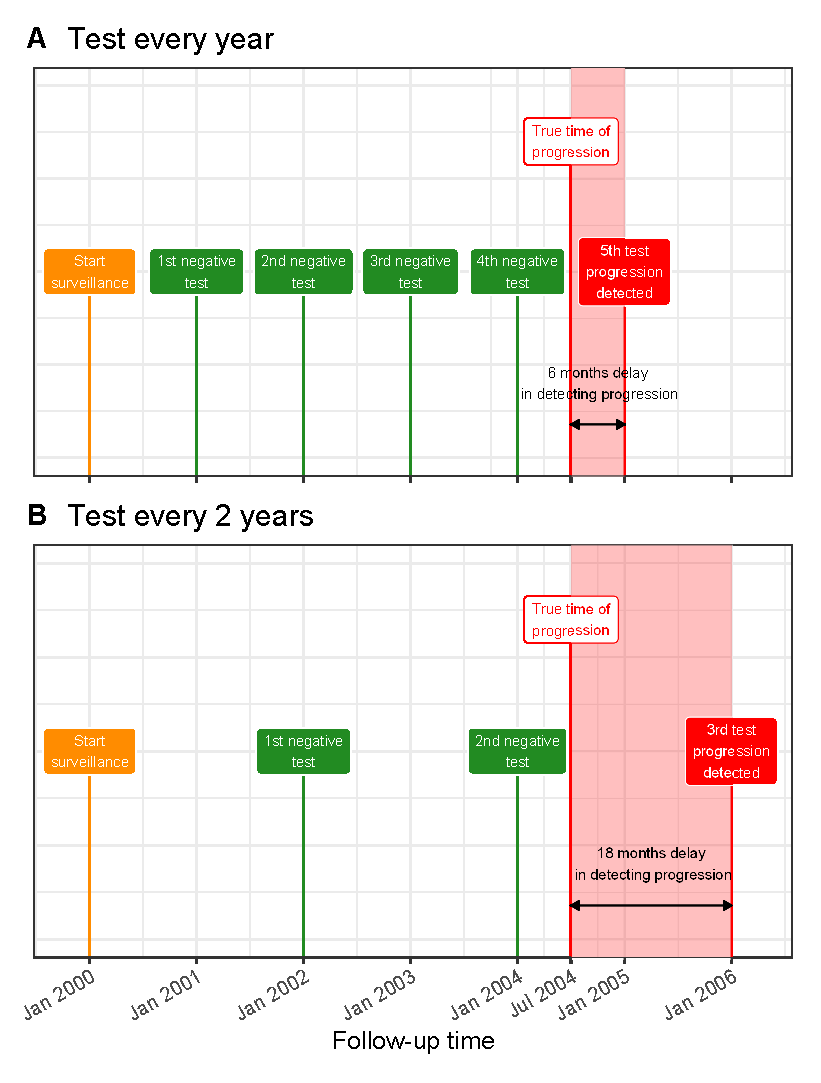
\includegraphics{delay_explanation.eps}}
\caption{\textbf{Goal: Finding the optimal tradeoff between the number of invasive tests (burden) and time delay in detecting progression (shorter is beneficial)}. A progression is a non-terminal event in the surveillance of early-stage chronic non-communicable diseases. The true time of progression for the patient illustrated in this figure is July 2004. Since invasive tests are conducted repeatedly, progression is interval-censored and always observed with a delay. Frequent periodical invasive tests in \textbf{Panel~A} lead to a shorter time delay in detecting progression than infrequent periodical invasive tests in \textbf{Panel~B}. The interval-censored time of progression is Jan~2004--Jan~2005 in \textbf{Panel~A} and between Jan~2004--Jan~2006 in \textbf{Panel~B}.} 
\label{fig:delay_explanation}
\end{figure}

The goal of this work (Figure~\ref{fig:delay_explanation}) is to optimize the number of invasive tests and the time delay in detecting progression better than fixed schedules. Specifically, we intend to \emph{personalize} test schedules using patients' clinical data accumulated over surveillance follow-up. This data includes baseline characteristics; previous invasive test results; and longitudinal outcomes such as biomarkers, physical examination, and medical imaging measurements. Previous attempts at personalized scheduling can be divided into three categories. First, heuristic approaches such as decision making flowcharts~\citep{bokhorst2015compliance,weusten2017endoscopic}. However, flowcharts discretize continuous clinical outcomes, often exploit only the last measurement, and ignore the measurement error in observed data. Second, partially observable Markov decision processes~\citep{alagoz2010operations, steimle2017markov} for personalizing test decisions. Although the curse of dimensionality limits their application with continuous longitudinal outcomes. Third, personalized schedules may be obtained by optimizing an explicit utility function of the clinical parameters of interest~\citep{bebu2017optimal,rizopoulos2015personalized}, including our previous work on scheduling biopsies in prostate cancer~\citep{tomer2019personalized,tomer2020webapp}. In this work, we will employ the third approach.

Our solution is as follows. We first develop a full specification of the joint distribution of the patient-specific longitudinal outcomes and the time of progression. To this end, we utilize joint models for time-to-event and longitudinal data~\citep{tsiatis2004joint,rizopoulos2012joint} because they are inherently personalized. Specifically, joint models utilize patient-specific random effects~\citep{mcculloch2005generalized} to model longitudinal outcomes without discretizing them. Subsequently, we input the accumulated clinical data of a new patient into the fitted model to obtain their patient-specific cumulative-risk of progression at their current and future follow-up visits. We then create personalized schedules by planning tests on future visits where the predicted conditional cumulative-risk is above a particular \emph{threshold} (e.g., 5\% risk). We automate the choice of this threshold and the resulting schedule. In particular, we optimize a utility function of the expected number of tests (burden) and time delay in detecting progression (shorter is beneficial) for personalized schedules based on different risk thresholds. We estimate these two quantities for any given schedule in a patient-specific manner using the predicted risk profile of the patient. Hence, patients/doctors can compare the consequences of opting for personalized versus fixed schedules objectively.

%\subsection{Motivational Study}
%\label{subsec:motivational_study}
Our motivation comes from the problem of scheduling biopsies in the world's largest prostate cancer surveillance, called prostate cancer research international active surveillance~\citep{bokhorst2015compliance}, or PRIAS. It has 7813 patients (1134 progressions) with 104904 longitudinal measurements~\citep{tomer2020webapp}. These patients have low/very-low grade cancer, often over-diagnosed due to prostate-specific antigen (PSA) based screening~\citep{loeb2014overdiagnosis}. Surveillance aims to delay serious treatments (e.g., surgery, radiotherapy) until progression is observed. Consequently, patients are monitored routinely via PSA (ng/mL), digital rectal examination or DRE (tumor shape/size), and biopsy Gleason grade group~\citep{epsteinGG2014}. Among these, a biopsy Gleason grade group~$\geq$ 2 is the reference test for confirming progression. Most often, biopsies are scheduled annually~\citep{loeb2014heterogeneity}. However, such a frequent schedule can put an unnecessary burden on patients with slow/non-progressing cancers and cause non-compliance~\citep{bokhorst2015compliance}. Since prostate cancer has the second-highest incidence among all cancers in males~\citep{GlobalCancerStats2012}, individualized biopsy schedules can reduce the burden of biopsies in numerous patients worldwide.

The remaining paper is as follows. Section~\ref{sec:jointmodel} introduces the joint modeling framework. We describe the personalized scheduling methodology in Section~\ref{sec:schedule}, and demonstrate them for prostate cancer surveillance patients in Section~\ref{sec:results}. In Section~\ref{sec:sim_study}, we compare personalized and fixed schedules via a simulation study based on a joint model fitted to the PRIAS dataset.

% !TEX root =  ../main_manuscript.tex 
\section{Joint Model for Time-to-Progression and Longitudinal Outcomes}
\label{sec:jointmodel}
Let $T_i^*$ denote the true time of disease progression for the ${i\mbox{-th}}$ patient. Progression is always interval censored ${l_i < T_i^* \leq r_i}$ (Figure~\ref{fig:delay_explanation}). Here, $r_i$ and $l_i$ denote the time of the last and second last invasive tests, respectively, when patients progress. In non-progressing patients, $l_i$ denotes the time of the last test and ${r_i=\infty}$. Assuming $K$ types of longitudinal outcomes, let $\boldsymbol{y}_{ki}$ denote the ${n_{ki} \times 1}$ longitudinal response vector of the ${k\mbox{-th}}$ outcome, $k \in \{1, \ldots, K\}$. The observed data of all $n$ patients is given by ${\mathcal{A}_n = \{l_i, r_i, \boldsymbol{y}_{1i},\ldots \boldsymbol{y}_{Ki}; i = 1, \ldots, n\}}$.

\subsection{Longitudinal Sub-process}
To model different longitudinal outcomes in a unified framework, a joint model employs individual generalized linear mixed sub-models~\citep{mcculloch2005generalized}. Specifically, the conditional distribution of the $k$-th outcome $\boldsymbol{y}_{ki}$ given a vector of patient-specific random effects $\boldsymbol{b}_{ki}$ is assumed to belong to the exponential family, with linear predictor given by,
\begin{equation*}
\label{eq:long_model}
g_k\big[E\{y_{ki} (t) \mid \boldsymbol{b}_{ki}\}\big] = m_{ki}(t) = \boldsymbol{x}_{ki}^{\top}(t)\boldsymbol{\beta}_{k} + \boldsymbol{z}_{ki}^{\top}(t)\boldsymbol{b}_{ki},
\end{equation*}
where $g_k(\cdot)$ denotes a known one-to-one monotonic link function, $y_{ki}(t)$ is the
value of the ${k\mbox{-th}}$ longitudinal outcome for the ${i\mbox{-th}}$ patient at time $t$, and $\boldsymbol{x}_{ki}(t)$ and $\boldsymbol{z}_{ki}(t)$ are the time-dependent design vectors for the fixed $\boldsymbol{\beta}_{k}$ and random effects $\boldsymbol{b}_{ki}$, respectively. To model the correlation between different longitudinal outcomes, we link their corresponding random effects. Specifically, the complete vector of random effects ${\boldsymbol{b}_{i} = (\boldsymbol{b}_{1i}^{\top}, \ldots, \boldsymbol{b}_{Ki}^{\top})^{\top}}$ is assumed to follow a multivariate normal distribution with mean zero and variance-covariance matrix $W$.

\subsection{Survival Sub-process}
\label{subsec:surival_sub_model}
In the survival sub-process, hazard of progression $h_i(t)$ at a time $t$ is assumed to depend on a function of patient and outcome-specific linear predictors $m_{ki}(t)$ and/or the random effects:
\begin{equation*}
\label{eq:rel_risk_model}
h_i\big\{t \mid \mathcal{M}_i(t), \boldsymbol{w}_i(t)\big\} = h_0(t) \exp\Big[\boldsymbol{\gamma}^{\top}\boldsymbol{w}_i(t) + \sum_{k=1}^{K} f_{k} \big\{ \mathcal{M}_{ki}(t), \boldsymbol{w}_i(t), \boldsymbol{b}_{ki}, \boldsymbol{\alpha}_{k} \big\}\Big], \quad t>0,
\end{equation*}
where $h_0(\cdot)$ denotes the baseline hazard, $\mathcal{M}_{ki}(t)=\{m_{ki}(s) \mid 0 \leq s < t \}$ is the history of the ${k\mbox{-th}}$ longitudinal process up to $t$, and $\boldsymbol{w}_i(t)$ is a vector of exogenous, possibly time-varying covariates with regression coefficients $\boldsymbol{\gamma}$. Functions $f_{k}(\cdot)$, parameterized by vector of coefficients $\boldsymbol{\alpha_{k}}$, specify the features of each longitudinal outcome that are included in the linear predictor of the relative-risk model~\citep{brown2009assessing,rizopoulos2012joint,taylor2013real}. Some examples, motivated by the literature (subscripts $k$ dropped for brevity), are:
\begin{eqnarray*}
\left \{
\begin{array}{l}
f\big\{\mathcal{M}_{i}(t), \boldsymbol{w}_i(t), \boldsymbol{b}_{i}, \boldsymbol{\alpha} \big\} = \alpha m_{i}(t),\\
f\big\{ \mathcal{M}_{i}(t), \boldsymbol{w}_i(t), \boldsymbol{b}_{i}, \boldsymbol{\alpha}\big\} = \alpha_1 m_{i}(t) + \alpha_2 m'_{i}(t),\quad \text{with}\  m'_{i}(t) = \frac{\mathrm{d}{m_{i}(t)}}{\mathrm{d}{t}}.\\
\end{array}
\right.
\end{eqnarray*}
These formulations of $f(\cdot)$ postulate that the hazard of progression at time $t$ may depend on underlying level $m_i(t)$ of the longitudinal outcome at $t$, or on both the level and velocity $m'_i(t)$ (e.g., PSA value and velocity in prostate cancer) of the outcome at $t$. Lastly, the baseline hazard $h_0(t)$ is modeled flexibly using P-splines~\citep{eilers1996flexible}. The detailed specification of the baseline hazard, and the joint parameter estimation of the longitudinal and relative-risk sub-models using the Bayesian approach are presented in Web-Appendix~A.

% !TEX root =  ../main_manuscript.tex 
\section{Personalized Schedule of Invasive Tests for Detecting Progression} 
\label{sec:schedule}

\subsection{Cumulative-risk of progression} 
\label{subsec:cum_risk}
Using the joint model fitted to the training data $\mathcal{A}_n$, we aim to derive a personalized schedule of invasive tests for a new patient $j$ with true progression time $T^*_j$. For this purpose, our calculations are based on the dynamic \emph{cumulative-risk} function. Let $t < T^*_j$ be the time of the last conducted test at which progression was not observed. Let $\{\mathcal{Y}_{1j}(v), \ldots, \mathcal{Y}_{Kj}(v)\}$ denote the history of observed longitudinal data up to the current visit time $v$. The current visit can be after the last negative test, i.e., $v \geq t$ (e.g., PSA after negative biopsy in prostate cancer). The cumulative-risk of progression for patient $j$ at future time $u$ is then defined as:
\begin{equation}
\label{eq:cumulative_risk}
\begin{split}
R_j(u \mid t, v) &= \mbox{Pr}\big\{T^*_j \leq u \mid T^*_j > t, \mathcal{Y}_{1j}(v), \ldots, \mathcal{Y}_{Kj}(v), \mathcal{A}_n\big\}\\
&=\int \int \mbox{Pr}(T^*_j \leq u \mid T^*_j > t, \boldsymbol{b}_{j}, \boldsymbol{\theta}) p\big\{\boldsymbol{b}_j \mid T^*_j > t, \mathcal{Y}_{1j}(v), \ldots, \mathcal{Y}_{Kj}(v), \boldsymbol{\theta} \big\}\\
&\quad \times p(\boldsymbol{\theta} \mid \mathcal{A}_n) \mathrm{d}\boldsymbol{b}_j \mathrm{d}\boldsymbol{\theta}, \quad u \geq t.
\end{split}
\end{equation}
The cumulative-risk function $R_j(\cdot)$ depends on patient-specific clinical data and the training dataset, via the posterior distribution of the random effects $\boldsymbol{b}_{j}$ and posterior distribution of the vector of all parameters $\boldsymbol{\theta}$ of the fitted joint model, respectively. This cumulative-risk function is dynamic, in the sense that it automatically updates over time as more longitudinal data become available (Figure~\ref{fig:dynrisk_explanation}).
\begin{figure}
\centerline{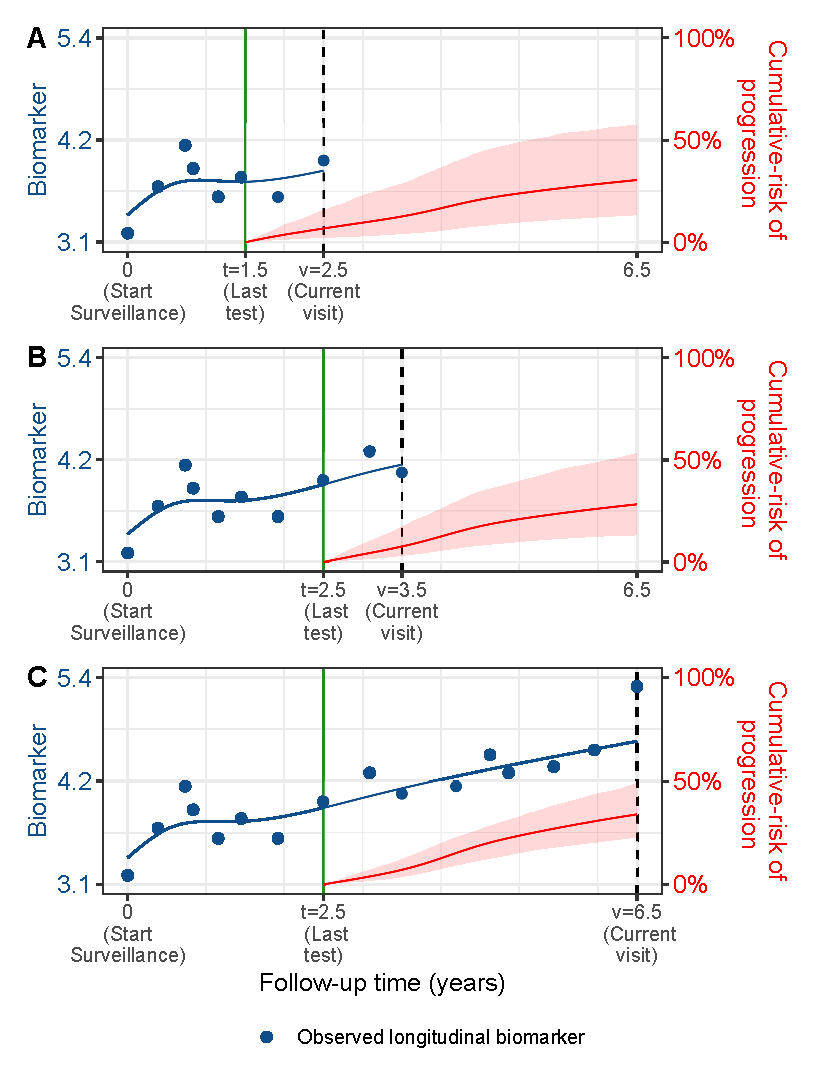
\includegraphics{dynrisk_plot_102.eps}}
\caption{\textbf{Cumulative-risk of progression updated dynamically over follow-up} as more patient data is gathered. A single longitudinal outcome, namely, a continuous biomarker of disease progression, is used for illustration. \textbf{Panels~A,~B~and~C:} are ordered by the time of the current visit $v$ (dashed vertical black line) of a new patient. At each of these visits, we combine the accumulated longitudinal data (shown in blue), and time of the last negative invasive test $t$ (solid vertical green line) to obtain the updated cumulative-risk profile $R_j(u \mid t, v)$ (shown in red) of the patient defined in~(\ref{eq:cumulative_risk}). All values are illustrative.}\label{fig:dynrisk_explanation}
\end{figure}

\subsection{Personalized Test Decision Rule} 
\label{subsec:pers_schedule}
We intend to exploit the cumulative-risk function $R_j(\cdot)$ to develop a risk-based personalized schedule of invasive tests for the $j$-th patient. Typically, invasive tests are decided on the same visit times on which longitudinal data (e.g., biomarkers) are measured. Let $U = \{u_1, \ldots, u_L\}$ represent a schedule of such visits (e.g., biannual PSA measurement in prostate cancer).  Here, $u_1 = v$ is also the current visit time. The maximum future visit time $u_L$ can be chosen based on the available information in the training dataset $\mathcal A_n$. That is, tests for the new patient $j$ are planned only up to a future visit time $u_L$ at which a sufficient number of events in $\mathcal A_n$ are available (e.g., up to the 80\% or 90\% percentile of progression times).

We propose to take the decision of conducting a test at a future visit time $u_l \in U$ if the cumulative-risk of progression at time $u_l$ exceeds a certain risk threshold $\kappa$ (Figure~\ref{fig:schedule_explanation}). In particular, the test decision at time $u_l$ is given by,
\begin{equation}
\label{eq:personalized_decision_grid}
Q_j^\kappa (u_l \mid t_l, v) = I \big \{ R_j(u_l \mid t_l, v) \geq \kappa \big\}, \quad 0 \leq \kappa \leq 1,
\end{equation}
where $I(\cdot)$ is the indicator function, $R_j(u_l \mid t_l, v)$ is the cumulative-risk of progression at the current decision time $u_l$, and $t_l < u_l$ is the time of the last test conducted before $u_l$. Thus, the future time at which a test will be planned, depends on both the threshold $\kappa$ and the cumulative-risk of the patient. In this regard, when a test gets planned at time $u_l$, i.e., $Q_j^\kappa (u_l \mid t_l, v) = 1$, then the cumulative-risk profile is updated before making the next test decision at time $u_{l+1}$ (Figure~\ref{fig:schedule_explanation}). Specifically, the cumulative-risk at time $u_{l+1}$ is updated by setting the corresponding time of the last test $t_{l+1}=u_l$. This accounts for the possibility that progression may occur after time $u_l < T^*_j$. Hence, the time of last test $t_l$ is defined as,
\begin{equation*}
t_l = \left \{ 
\begin{array}{ll}
t, & \mbox{if } l = 1,\\
u_{l-1}, & \mbox{if } l \geq 2 \mbox{ and } Q_j^\kappa (u_{l-1} \mid t_{l-1}, v) = 1,\\
t_{l-1}, & \mbox{if } l \geq 2 \mbox{ and } Q_j^\kappa (u_{l-1} \mid t_{l-1}, v) = 0.\\
\end{array}
\right.
\end{equation*}
We should note that in all future test decisions, we use only the observed longitudinal data up to the current visit time $v$, i.e., $\{\mathcal Y_{1j}(v), \ldots, Y_{Kj}(v)\}$.
\begin{figure}
\centerline{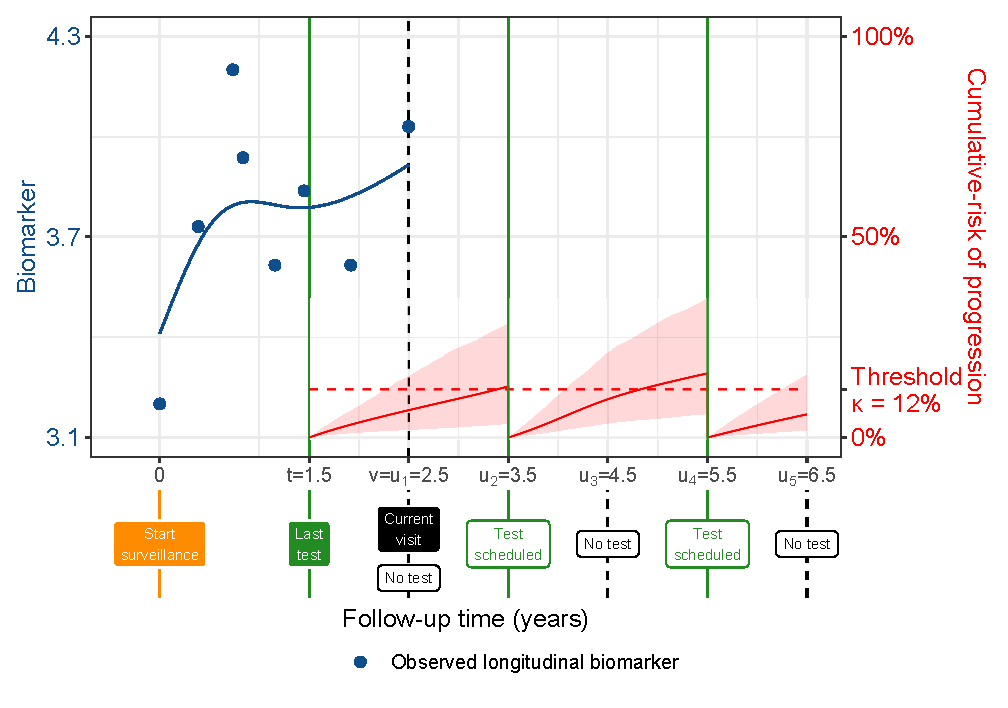
\includegraphics{schedule_explanation_102.eps}}
\caption{\textbf{Successive personalized test decisions~(\ref{eq:personalized_decision_grid}) based on patient-specific cumulative-risk of progression}. Time of current visit: $v=2.5$ years (black dashed line). Time of the last test on which progression was not observed: $t=1.5$ years. Longitudinal data up to current visit: $\mathcal{Y}_j(v)$ is a continuous biomarker (observed: blue dots, fitted: blue line). Example risk threshold: $\kappa=0.12$ (12\%). Grid of future visits on which future tests are planned: $U = \{2.5, 3.5, 4.5, 5.5, 6.5\}$ years. The cumulative-risk profiles $R_j(u_l \mid t_l, v)$ employed in~(\ref{eq:personalized_decision_grid}) are shown with red line (95\% credible interval shaded), and are updated each time a test is planned. Future test decisions $Q_j(u_l \mid t_l, v)$ defined in~(\ref{eq:personalized_decision_grid}) are: $Q_j^\kappa(u_1=2.5\mid t_1=1.5,v)=0$, $Q_j^\kappa(u_2=3.5\mid t_2=1.5,v)=1$, $Q_j^\kappa(u_3=4.5\mid t_2=3.5,v)=0$, $Q_j^\kappa(u_4=5.5\mid t_2=3.5,v)=1$, and $Q_j^\kappa(u_5=6.5\mid t_5=4.5,v)=0$. All values are illustrative.} 
\label{fig:schedule_explanation}
\end{figure}

\subsection{Expected Number of Tests and Expected Time Delay in Detecting Progression}
\label{subsec:exp_delay_estimation}
To facilitate shared-decision making of invasive tests, we translate our proposed decision rule, i.e., the choice of a specific risk threshold $\kappa$, into two clinically relevant quantities. First, the number of tests (burden) we expect to perform for patient $j$, and second, if the patient progresses, the time delay (shorter is beneficial) expected in detecting progression. To calculate these two quantities, we first suppose that patient $j$ does not progress between his last negative test at time $t$ and the maximum future visit time $u_L$. Under this assumption, the subset of future visit times in $U$ on which a test is planned using~(\ref{eq:personalized_decision_grid}) results into a personalized schedule of future tests (Figure~\ref{fig:schedule_explanation}), given by:
\begin{equation}
\label{eq:personalized_schedule_grid}
\{s_1, \ldots, s_{N_j}\} = \big\{ u_l \in U : Q_j^\kappa(u_l \mid t_l, v) = 1 \big\}, \quad N_j \leq L.
\end{equation}

If patient $j$ never progressed in the period $[t, u_L]$, as we initially supposed, all $N_j$ tests in $\{s_1, \ldots, s_{N_j}\}$ will be conducted. However, fewer tests will be performed if the patient did progress at some point $T_j^* < u_L$. We formally define the discrete random variable $\mathcal{N}_j$ denoting the number of performed tests in conjunction with the true progression time $T_j^*$ as:
\[
\mathcal{N}_j (S^\kappa_j) = \left \{
\begin{array}{ll}
1, & \mbox{ if } \; t < T^*_j \leq s_1,\\
2, & \mbox{ if } \; s_1 < T^*_j \leq s_2,\\
\vdots&\\
N_j, & \mbox{ if } \; s_{N_j-1} < T^*_j \leq s_{N_j},
\end{array}
\right.
\]
where $S^\kappa_j = \{s_1, \ldots, s_{N_j}\}$ is the schedule of planned future tests. The expected number of future tests for patient $j$ will be the expected value $E \big \{\mathcal N_j(S^\kappa_j)\big\}$, given by the expression:
\begin{equation*}
\label{eq:exp_tests}
E \big \{\mathcal N_j(S^\kappa_j)\big\} = \sum_{n = 1}^{N_j} n \times \mbox{Pr}(s_{n-1} < T^*_j \leq s_n \mid T^*_j \leq s_{N_j}), \quad s_0 = t,
\end{equation*}
where 
\begin{equation*}
\mbox{Pr}(s_{n-1} < T^*_j \leq s_n \mid T^*_j \leq s_{N_j}) = \frac{R_j(s_n \mid t, v) - R_j(s_{n-1} \mid t, v)}{R_j(s_{N_j} \mid t, v)}.
\end{equation*}

Similarly, we can define the expected time delay in detecting progression, under the assumption that progression occurs before $u_L$. Specifically, the random variable time delay is equal to the difference between the time of the test at which progression is observed and the true time of progression $T_j^*$, and is given by:
\[
\mathcal D_j (S^\kappa_j) = \left \{
\begin{array}{ll}
s_1 - T_j^*, & \mbox{ if } \; t < T^*_j \leq s_1,\\
s_2 - T_j^*, & \mbox{ if } \; s_1 < T^*_j \leq s_2,\\
\vdots&\\
s_{N_j} - T_j^*, & \mbox{ if } \; s_{N_j-1} < T^*_j \leq s_{N_j},
\end{array}
\right.
\]
The expected time delay in detecting progression is the expected value of $\mathcal D_j (S^\kappa_j)$, given by the expression:
\begin{equation*}
\label{eq:exp_delay}
E \big \{ \mathcal D_j(S^\kappa_j)\big\} = \sum_{n = 1}^{N_j} \Big\{s_n - E(T^*_j \mid s_{n-1}, s_n, v)\Big\} \times \mbox{Pr}(s_{n-1} < T^*_j \leq s_n\mid T^*_j \leq s_N),
\end{equation*}
where $E(T^*_j \mid s_{n-1}, s_n, v)$ denotes the conditional expected time of progression for the scenario $s_{n-1} < T^*_j \leq s_n$ and is calculated as the area under the corresponding survival curve,
\begin{equation*}
E(T^*_j \mid s_{n-1}, s_n, v) = s_{n-1} + \int_{s_{n-1}}^{s_n} \mbox{Pr}\Big\{T^*_j \geq u \mid s_{n-1} < T^*_j \leq s_n, \mathcal{Y}_{1j}(v), \ldots, \mathcal{Y}_{Kj}(v), \mathcal{A}_n\Big\} \mathrm{d}u.
\end{equation*}

The personalized schedule in~(\ref{eq:personalized_schedule_grid}), and the corresponding personalized expected number of tests and time delay, have the advantage of getting updated with newly collected data over follow-up. Also, the expected number of tests and time delay can be calculated for any schedule, fixed or personalized. Hence, patients/doctors can use them to compare different schedules. Although, a fair comparison of time delays between different schedules for the same patient, requires a compulsory test at a common horizon time point in all schedules.

\subsection{How to Select the Risk Threshold $\kappa$}
\label{subsec:kappa_selection}
The risk threshold $\kappa$ controls the timing and the total number of invasive tests in the personalized schedule $S^\kappa_j$. Through the timing and the total number of planned tests, $\kappa$ also indirectly affects the time delay (Figure~\ref{fig:delay_explanation}) that may occur in detecting progression if a particular schedule is followed. Hence, $\kappa$ should be chosen while balancing both the number of invasive tests (burden) and the time delay in detecting progression (shorter is beneficial).

To facilitate the choice of $\kappa$ in practice, following our developments in the previous section, we translate the different choices for threshold $\kappa$ into the expected number of tests and time delay. In particular, for a patient $j$ having data available up to his current visit time $v$, we can construct a bi-dimensional Euclidean space of his expected total number of tests (x-axis) and expected time delay in detecting progression (y-axis), for different personalized test schedules obtained by varying $\kappa$ in $[0, 1]$. An example of such a space is given in Figure~\ref{fig:kappa_choice}.
\begin{figure}
\centerline{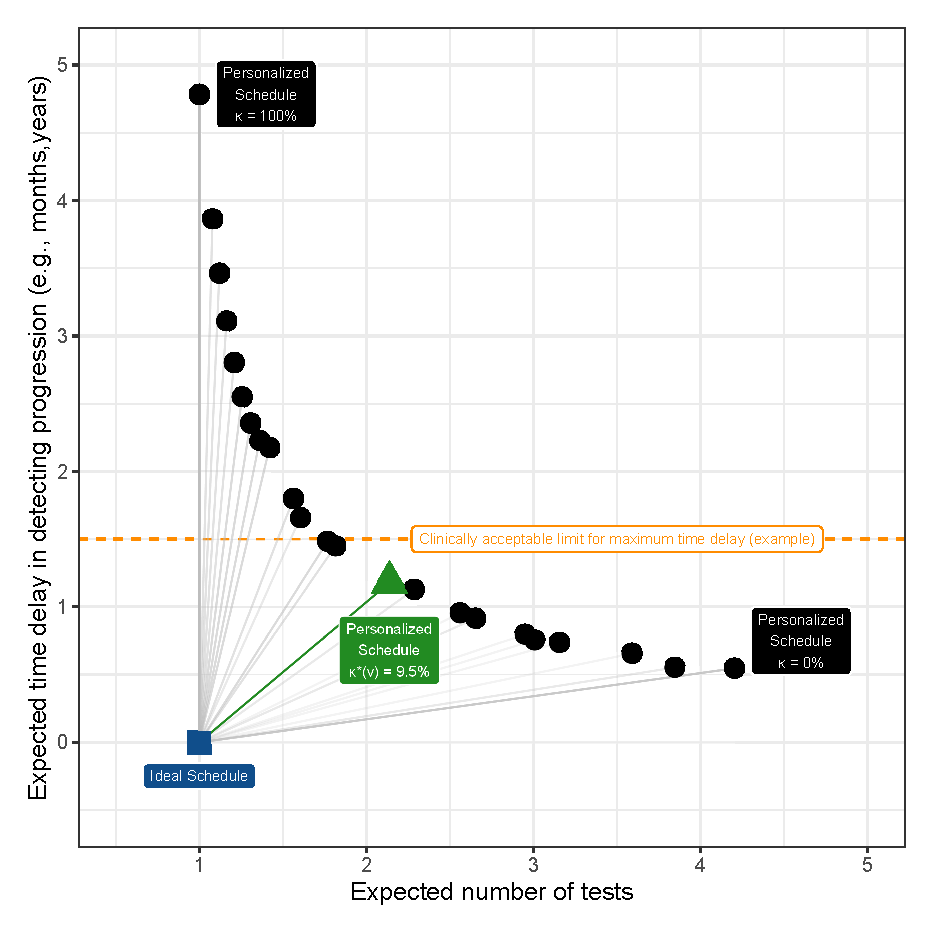
\includegraphics{kappa_choice_102.eps}}
\caption{\textbf{Optimal current-visit time $v$ specific risk threshold $\kappa^*(v)$ obtained using~(\ref{eq:kappa_choice})} for the patient shown in Figure~\ref{fig:schedule_explanation}. Ideal schedule of tests: point (1,0) shown as a blue square. It plans exactly one invasive test at the true time of progression $T^*_j$ of a patient. Hence, the time delay in detecting progression is zero. Various personalized schedules based on a grid of thresholds $\kappa$ in $[0,1]$ are shown with black circles. Higher thresholds lead to fewer tests, but also higher expected time delay. The personalized schedule based on $\kappa^*(v)=9.5\%$ threshold (green triangle) has the least Euclidean distance (shown with a green line) to the ideal schedule. It is also possible to optimize the least distance under a certain clinically acceptable limit on the time delay (orange dashed line).}
\label{fig:kappa_choice}
\end{figure}

The ideal schedule for $j$-th patient is the one in which only one test is conducted, at exactly the true time of progression $T^*_j$. In other words, the time delay will be zero. If we weigh the expected number of tests and time delay as equally important, then we can select as the optimal threshold at current visit time $v$, the threshold $\kappa^*(v)$ which minimizes the Euclidean distance between the ideal schedule, i.e., point (1, 0) and the set of points representing the different personalized schedules $S^{\kappa}_j$ corresponding to various $\kappa \in [0, 1]$, i.e.,
\begin{equation}
\label{eq:kappa_choice}
\kappa^*(v) = \argmin_{0 \leq \kappa \leq 1} \sqrt{\Big[E\big\{\mathcal N_j(S^\kappa_j)\big\} - 1\Big]^2 + \Big[E\big\{\mathcal D_j(S^\kappa )\big\} - 0\Big]^2}.
\end{equation}
In certain scenarios, patients/doctors may be apprehensive about undergoing more than a maximum expected number of future tests, or having an expected time delay higher than certain months. For such purposes, the Euclidean distance in ~(\ref{eq:kappa_choice}) can be optimized under constraints on the expected number of tests or expected time delay (Figure~\ref{fig:kappa_choice}). Doing so alleviates two problems, namely, that the time delay and the number of tests have different units of measurement, and that in~(\ref{eq:kappa_choice}) they are weighted equally~\citep{cook1994equivalence}.

We considered shorter delays in detecting progression as the benefit of repeated tests. However, it is also common to describe the benefit of testing in terms of decision-theoretic measures such as quality-adjusted life-years/expectancy (QALY/QALE) gained~\citep{sassi2006calculating}. Optimizing~(\ref{eq:kappa_choice}) with QALE needs, setting the optimal point in a Euclidean space with QALE as a dimension, and obtaining expected QALEs for different schedules. For estimating the expected QALE in a personalized manner, a mathematical definition of QALE in terms of time delay $\mathcal{D}_j$ in detecting progression~\citep{de2017should} is required.

% !TEX root =  ../main_manuscript.tex 
\section{Application of Personalized Schedules in Prostate Cancer Surveillance}
\label{sec:results}
We next demonstrate personalized schedules for scheduling biopsies in prostate cancer active surveillance. To this end, we reuse results from a joint model we previously fitted~\citep{tomer2019personalized} to the PRIAS dataset introduced in Section~\ref{sec:introduction}. This model utilized a linear mixed sub-model for biannually measured PSA (continuous: log-transformed from ng/mL), and a logistic mixed sub-model for biannually measured DRE (binary: tumor palpable or not). The model employed B-splines~\citep{de1978practical} to accommodate non-linear PSA evolution over follow-up. In the survival sub-model, fitted PSA value, fitted instantaneous PSA velocity (defined in Section~\ref{subsec:surival_sub_model}), and log-odds of having a DRE indicating a palpable tumor, were included as time-dependent predictors. The model parameters were estimated under the Bayesian framework~\citep{tomer2019personalized} using the R package \textbf{JMbayes}~\citep{rizopoulosJMbayes}. While the complete model definition and parameter estimates are provided in~\citet{tomer2019personalized}, we next briefly present the key results relevant for personalized scheduling.

First, the cause-specific cumulative-risk of cancer progression at the maximum study period of ten years was 50\% (Web-Figure~1). This indicates that many patients may not require all of the yearly biopsies they are usually prescribed. Since personalized schedules are risk-based, their overall performance is dependent on the predictive accuracy and discrimination capacity of the fitted model. In this regard, the model had a moderate area under the receiver operating characteristic curve (AUC) over the follow-up period (between 0.61 and 0.68). The mean absolute prediction error was moderate to large (between 0.08 and 0.24) and decreased rapidly after year one of the follow-up. Thus, personalized schedules based on this model may work better after year one with more follow-up data.

\subsection{Personalized Biopsy Schedules for a Demonstration Prostate Cancer Patient}
\label{subsec:demo_patient}
We utilized the joint model fitted to the PRIAS dataset to schedule biopsies in a demonstration prostate cancer patient shown in Figure~\ref{fig:demo_schedule}. The time of his last negative biopsy was $t=3.5$ years, and the time of the current visit was $v=5$ years. We made biopsy decisions over his future visits for PSA measurement $U=\{u_1=5, u_2=5.5,\ldots,u_L=10\}$ years using four different schedules. Two of the fixed schedules are annual biopsy schedule and the PRIAS schedule. The PRIAS schedule has compulsory biopsies at year one, four, seven, and ten of follow-up, and additional annual biopsies if PSA doubling-time~\citep{bokhorst2015compliance} is high. Remaining two schedules are personalized, namely, with a fixed threshold $\kappa=10\%$ risk, and an automatically chosen current visit time $v$ specific risk $\kappa^*(v)$ (Section~\ref{subsec:kappa_selection}). Since the demonstration patient's time of last negative biopsy $t=3.5$ is after year one of follow-up, a time delay in detecting progression
up to three years may not lead to adverse downstream outcomes~\citep{carvalho}.

\begin{figure}
\centerline{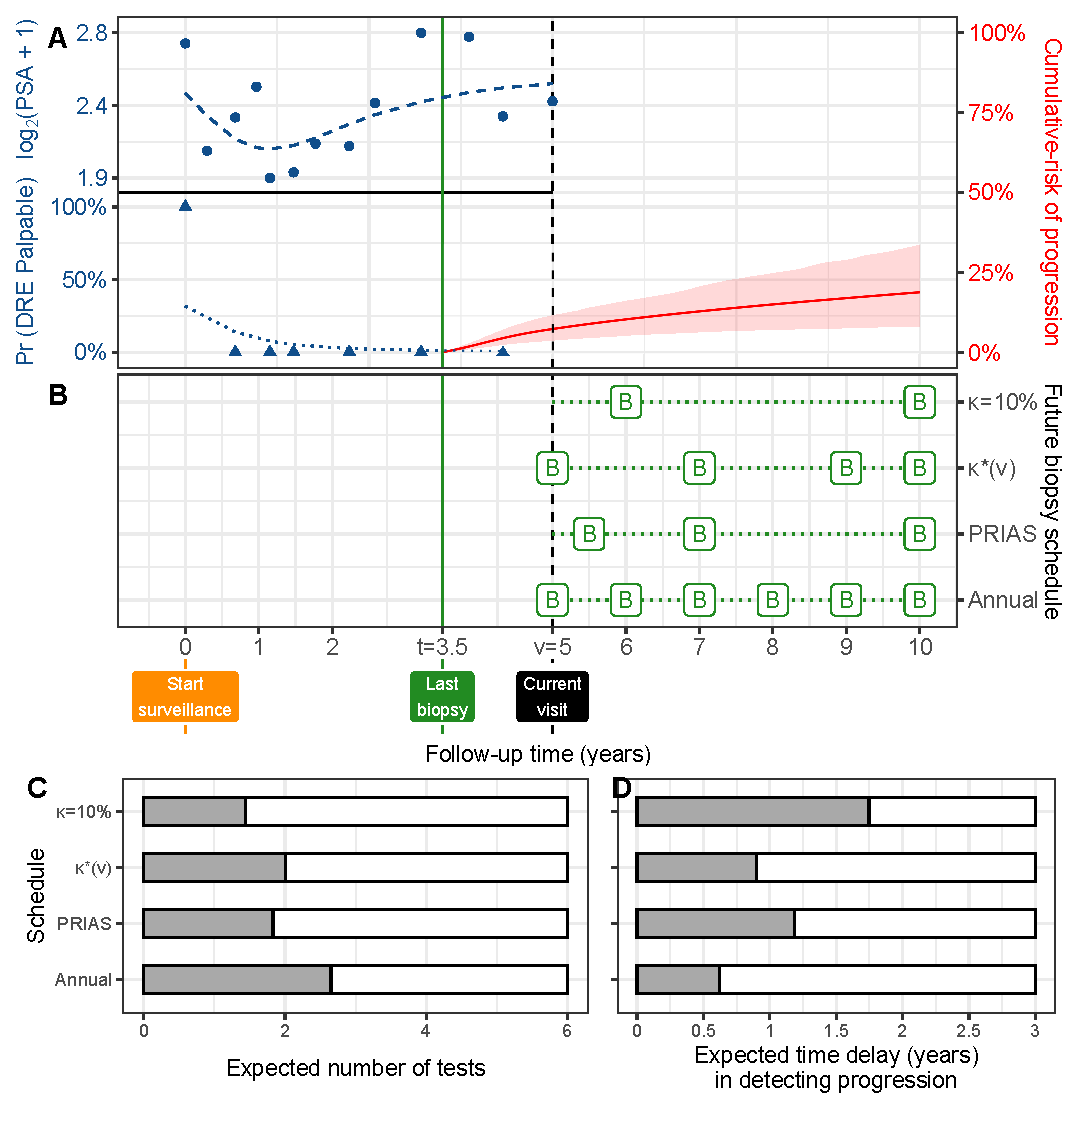
\includegraphics{demo_schedule.eps}}
\caption{\textbf{Personalized schedules for a demonstration prostate cancer patient}. \textbf{Panel~A}: Time of current visit: $v=5$ years (black dashed line). Time of last negative biopsy: $t=3.5$ years (vertical green solid line). Longitudinal data: $\log_2(\mbox{PSA} + 1)$ transformed~\citep{tomer2019personalized} PSA (observed: blue dots, fitted: dashed blue line), and binary DRE (observed: blue triangles, fitted probability: dotted blue line). Cumulative-risk profile: solid red line (95\% credible interval shaded). \textbf{Panel~B}: Different biopsy schedules are shown with a `B' indicating a biopsy. \textbf{$\kappa=10\%$} and \textbf{$\kappa^*(v)$} are personalized biopsy schedules using a risk threshold of 10\%, and a visit time $v$ specific automatically chosen threshold~(\ref{eq:kappa_choice}), respectively. PRIAS and Annual denote the PRIAS biopsy schedule (Section~\ref{subsec:demo_patient}) and annual biopsy schedule. \textbf{Panel~C,D}: For all schedules we calculate the expected number of tests and expected time delay in detecting progression if the patient progresses before year ten. Since a recommended minimum gap of one year is maintained between biopsies, maximum possible number of tests are six. A delay in detecting progression of up to three years may not lead to adverse outcomes~\citep{carvalho}. }
\label{fig:demo_schedule}
\end{figure}

The cumulative-risk of progression of the demonstration patient increases 3\% yearly on average, up to 19\% at the maximum study period of ten years. Hence, the patient may progress slowly. Consequently, risk-based personalized approaches plan fewer biopsies than the annual schedule (Panel~B, Figure~\ref{fig:demo_schedule}). Also, the time delay in detecting progression for personalized schedules (Panel~D, Figure~\ref{fig:demo_schedule}) is below the safe limit of three years mentioned earlier. Thus, personalized schedules can be a suitable alternative to the annual schedule.

\subsection{Web-application for Personalized Biopsy Schedules Prostate Cancer Surveillance}
We implemented the methodology for scheduling risk-based biopsies in prostate cancer active surveillance in a web-application (\textcolor{blue}{https://emcbiostatistics.shinyapps.io/prias\_biopsy\_recommender/}). In this web-application, four types of risk-based personalized schedules are provided, namely, using 5\%, 10\%, and 15\% fixed thresholds, and a current-visit time specific optimal threshold obtained via~(\ref{eq:kappa_choice}). Also, a general purpose source code for creating personalized test schedules is provided in Web-Appendix~D. The source code is compatible with joint models fitted using the R package \textbf{JMbayes}~\citep{rizopoulosJMbayes}.

% !TEX root =  ../main_manuscript.tex 
\section{Simulation Study}
\label{sec:sim_study}
Although we evaluated personalized schedules for a demonstration patient, we also intend to analyze and compare personalized and fixed schedules in a full cohort. Our criteria for comparison of schedules are the total number of invasive tests planned (burden), and the actual time delay in detecting progression (shorter is beneficial) for each schedule. Due to the periodical nature of schedules, the actual time delay in detecting progression cannot be observed in real-world surveillance. Hence, instead, we compare personalized versus fixed schedules via an extensive simulated randomized clinical trial in which each hypothetical patient undergoes each schedule. To keep our simulation study realistic, we employ the prostate cancer active surveillance scenario. Specifically, our simulated population is generated using the joint model fitted to the PRIAS cohort~\citep{tomer2019personalized}.

\subsection{Simulation Setup}
From the simulation population, we first sample 500 datasets, each representing a hypothetical prostate cancer surveillance program with 1000 patients in it. We generate a true cancer progression time for each of the ${\mbox{500} \times \mbox{1000}}$ patients, and then sample longitudinal DRE and PSA measurements biannually (PRIAS protocol) for them. We split each dataset into training (750 patients) and test (250 patients) parts, and generate a random and non-informative censoring time for the training patients. All training and test patients also observe Type-I censoring at year ten of follow-up (current study period of PRIAS). We next fit a joint model of the same specification as the model fitted to PRIAS~\citep{tomer2019personalized}, to each of the 500 training datasets and retrieve MCMC samples from the 500 sets of the posterior distribution of the parameters. In each of the 500 hypothetical surveillance programs, we utilize the corresponding fitted joint models to obtain the cumulative-risk of progression in each of the ${\mbox{500} \times \mbox{250}}$ test patients. These cumulative-risk profiles are further used to create personalized biopsy schedules for the test patients. 

For each test patient, we conduct hypothetical biopsies using two fixed (PRIAS and annual schedule) and three personalized biopsy schedules. Personalized schedules are based on, a fixed risk threshold $\kappa=10\%$, an optimal current visit time $v$ specific threshold $\kappa^*(v)$ chosen via~(\ref{eq:kappa_choice}), and an optimal threshold obtained under the constraint that expected time delay in detecting progression is less than 9 months (0.75 years), denoted $\kappa^*\{v \mid E(\mathcal{D})\leq 0.75\}$. Successive personalized biopsy decisions are made only on the standard PSA follow-up visits, utilizing clinical data accumulated only until the corresponding current visit time~(\ref{eq:personalized_decision_grid}). We maintain a minimum recommended gap of one year between consecutive prostate biopsies~\citep{bokhorst2015compliance} as well. Biopsies are conducted until progression is detected, or the maximum follow-up period at year ten (horizon) is reached. The actual time delay in detecting progression is equal to the difference in time at which progression is detected and the actual (simulated) time of progression of a patient.

\subsection{Simulation Results}
In the simulation study, nearly 50\% of the patients observed progression in ten year study period (\emph{progressing}) and 50\% did not (\emph{non-progressing}). While we can calculate the total number of biopsies scheduled in all $500 \times 250$ test patients, but the actual time delay in detecting progression is available only for progressing patients. Hence, we show the simulation results separately for progressing and non-progressing patients (Figure~\ref{fig:simulation_boxplot}).

Before discussing delay in detecting progression (Panel~A, Figure~\ref{fig:simulation_boxplot}), we note that mean delay up to 1.7 years in all patients~\citep{inoue2018comparative}, and up to three years in patients who progress after year one of follow-up~\citep{carvalho}, may not increase risks of adverse outcomes later. In this regard, the annual biopsies guarantee a maximum delay of one year in all patients. However, they also schedule the highest number of biopsies (Median~3, Inter-quartile range or IQR:~1--6). Much fewer biopsies are planned by the PRIAS schedule (Median~2, IQR:~1--4), but it also has a higher time delay (Median~0.74, IQR: 0.38--1.00 years). The personalized schedule based on optimal risk threshold $\kappa^*(v)$ schedules fewer biopsies than PRIAS and has a delay~(Median~0.86, IQR:~0.46--1.26 years) slightly higher than PRIAS. The expected delay for risk threshold optimized with a constraint on expected delay $\kappa^*\{v \mid E(D)\leq 0.75\}$ is equal to 0.61 years, i.e., the constraint works as expected.

The simulated non-progressing patients (Panel~B,~Figure~\ref{fig:simulation_boxplot}) gained the most with personalized schedules. The annual schedule plans 10 (unnecessary) biopsies for each such patient, and the PRIAS schedule plans a median of 6~(IQR:~4--8) biopsies. In contrast, the personalized schedule based on optimized risk threshold $\kappa^*(v)$ plans fewer biopsies consistently (Median~6, IQR:~6--7). The 10\% threshold based schedule plans even fewer biopsies (Median~5, IQR:~4--6).

\begin{figure}
\centerline{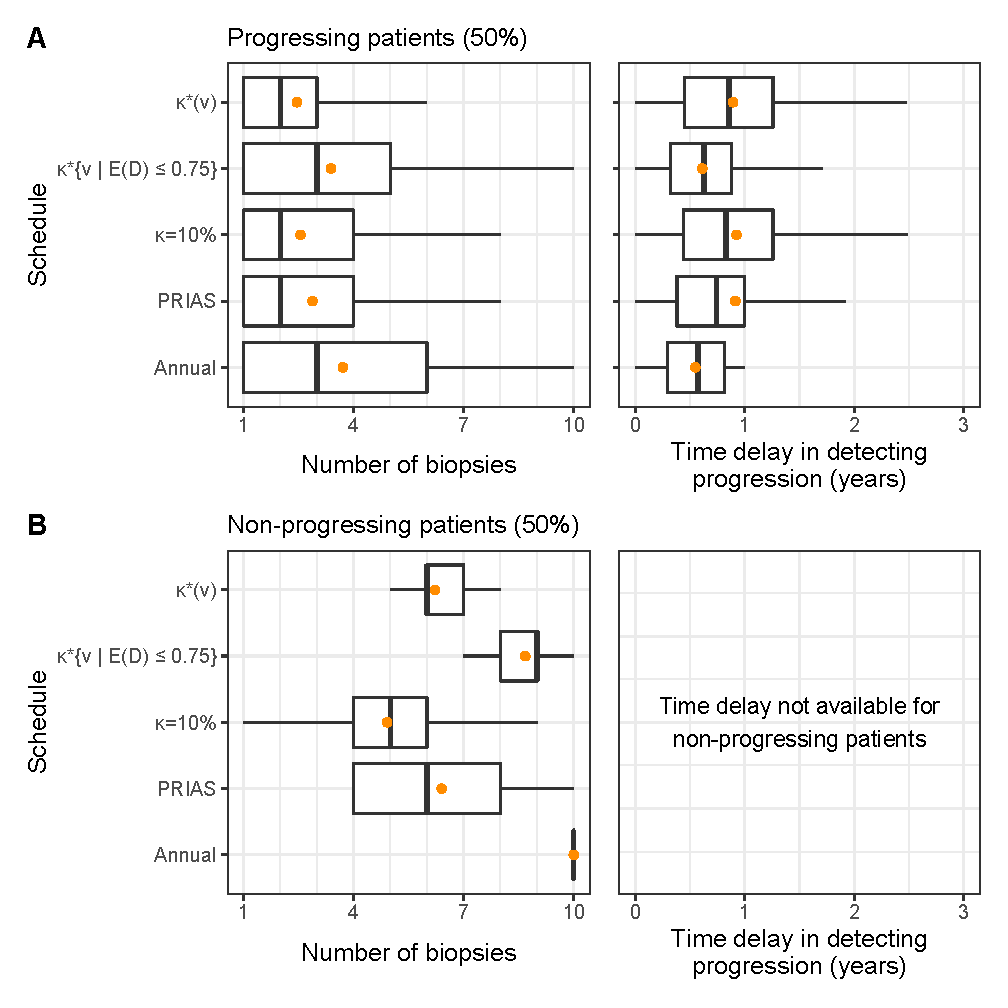
\includegraphics{simulation_boxplot.eps}}
\caption{\textbf{Number of biopsies and the time delay in detecting cancer progression for various biopsy schedules} obtained via a simulation study. \textbf{Mean} is indicated by the orange circle. Time delay (years) is calculated as (time of positive biopsy - the actual simulated time of cancer progression). Biopsies are conducted until cancer progression is detected. \textbf{Panel~A:} simulated patients who obtained cancer progression in the ten year study period (progressing). \textbf{Panel~B:} simulated patients who did not obtain cancer progression in the ten year study period (non-progressing). Types of schedules: ${\kappa=10\%}$ and $\kappa^*(v)$ schedule a biopsy if the cumulative-risk of cancer progression at the current visit time $v$ is more than 10\%, and an automatically chosen threshold~(\ref{eq:kappa_choice}), respectively. Schedule ${\kappa^*\{v \mid E(\mathcal{D})\leq 0.75\}}$ is similar to $\kappa^*(v)$ except that the euclidean distance in~(\ref{eq:kappa_choice}) is minimized under the constraint that expected delay in detecting progression is at most 9 months (0.75 years). Annual corresponds to a schedule of yearly biopsies, and PRIAS corresponds to biopsies as per PRIAS protocol (Section~\ref{sec:results}).}
\label{fig:simulation_boxplot}
\end{figure}

% !TEX root =  ../main_manuscript.tex 
\section{Discussion}
\label{sec:discussion}
In this paper, we presented a methodology to create personalized schedules for burdensome diagnostic \textit{tests} utilized to detect disease \textit{progression} in early-stage chronic non-communicable disease \textit{surveillance}. For this purpose, we utilized joint models for time-to-event and longitudinal data. Our approach first combines a patient's clinical data (e.g., longitudinal biomarkers) and previous invasive test results to estimate patient-specific cumulative-risk of disease progression over their current and future follow-up visits. We then plan future invasive tests whenever this cumulative-risk of progression is predicted to be above a certain threshold. We select the risk threshold automatically in a personalized manner, by optimizing a utility function of the patient-specific consequences of choosing a particular risk threshold based schedule. These consequences are, namely, the number of invasive tests (burden) planned in a schedule, and the expected time delay in detection of progression (shorter is beneficial) if the patient progresses. Last, we calculate this expected time delay in a personalized manner for both personalized and fixed schedules to assist patients/doctors in making a more informed decision of choosing a test schedule.

Using joint models gives us certain advantages. First, since joint models employ random-effects, the corresponding risk-based schedules are inherently personalized. Second, to predict this patient-specific risk of progression, joint models utilize all observed longitudinal measurements of a patient. Also, the continuous longitudinal outcomes are not discretized, which is commonly a case in Markov Decision Process and flowchart-based test schedules. Third, personalized schedules update automatically with more patient data over follow-up. Fourth, we calculated the expected number of tests (burden) and expected time delay in detecting progression (shorter is beneficial) in a patient-specific manner. Using our methodology, these can be calculated for both personalized and fixed schedules. Thus, patients/doctors can compare risk-based and fixed schedules and choose one according to their preferences for the expected burden-benefit ratio. Last, although this work concerns invasive test schedules in disease surveillance, the methodology is generic for use under a screening setting as well.

Personalized schedules that we proposed require a risk threshold. We optimized the threshold choice using a generic utility function based on the expected number of biopsies and time delay in detecting progression. We used only these two measures because they are easy to interpret but simultaneously critical for deciding the timing of invasive tests. Also, the time delay in detecting progression should manifest the window of opportunity for curative treatment and additional benefits of observing progression early. Practitioners may extend/modify this utility function by adding to/replacing time delay with commonly used decision-theoretic measures such as quality-adjusted life-years/expectancy (QALY/QALE).

We evaluated personalized schedules in a full cohort via a realistic simulation of a randomized clinical trial for prostate cancer surveillance patients. We observed that personalized schedules reduced many unnecessary biopsies for non-progressing patients compared to the widely used annual schedule. This happened at the cost of simultaneously having a slightly more time delay in detecting progression. Although, this delay should still be safe because it was almost equal to the delay of the world's largest prostate cancer active surveillance program PRIAS's schedule. The simulation study results are by no means the performance-limit of the personalized schedules. Instead, models with higher predictive accuracy and discrimination capacity than the PRIAS based model may lead to an even better balance between the number of tests and the time delay in detecting progression.

There are certain limitations to this work. First, in practice, most cohorts have a limited study period. Hence, the cumulative-risk profiles of patients and resulting personalized schedules can only be created up to the maximum study period. For this problem, the risk prediction model should be updated with more follow-up data over time. The proposed joint model assumed all events other than progression to be non-informative censoring. Alternative models that account for competing risks may lead to better results as they estimate absolute and not the cause-specific risk of progression. Upgrading is susceptible to inter-observer variation and sampling error. Although models that account for these two issues~\citep{balasubramanian2003estimation,coley2017prediction} will provide better risk estimates, the methodology for obtained personalized schedules can remain the same.

%  The \backmatter command formats the subsequent headings so that they
%  are in the journal style.  Please keep this command in your document
%  in this position, right after the final section of the main part of 
%  the paper and right before the Acknowledgements, Supporting Information (Supplementary %  Materials),   and References sections. 

\backmatter

%  This section is optional.  Here is where you will want to cite
%  grants, people who helped with the paper, etc.  But keep it short!

\section*{Acknowledgments}
The first and last authors would like to acknowledge support by Nederlandse Organisatie voor Wetenschappelijk Onderzoek (the national research council of the Netherlands) VIDI grant nr. 016.146.301, and Erasmus University Medical Center funding. Part of this work was carried out on the Dutch national e-infrastructure with the support of SURF Cooperative. The authors also thank the Erasmus University Medical Center's Cancer Computational Biology Center for giving access to their IT-infrastructure and software that was used for the computations and data analysis in this study. Last, we would like to thank the PRIAS consortium for enabling this research project.

\section*{Data Availability}
This work utilized results from a statistical model we previously fitted to the PRIAS dataset~\citep{tomer2019personalized}. The PRIAS database is not openly accessible. However, access to the database can be requested on the basis of a study proposal approved by the PRIAS steering committee. The website of the PRIAS program is \textcolor{blue}{www.prias-project.org}. For sake of completeness and reproducibility of results, we have presented the PRIAS based model's definition and parameter estimates in Web-Appendix~B. The data of the demonstration patient in Figure~\ref{fig:demo_schedule} is provided in Web-Appendix~B.

\section*{Supporting Information}
Web Appendices referenced in this paper are available in the file titled `supplementary.pdf'.

%  Here, we create the bibliographic entries manually, following the
%  journal style.  If you use this method or use natbib, PLEASE PAY
%  CAREFUL ATTENTION TO THE BIBLIOGRAPHIC STYLE IN A RECENT ISSUE OF
%  THE JOURNAL AND FOLLOW IT!  Failure to follow stylistic conventions
%  just lengthens the time spend copyediting your paper and hence its
%  position in the publication queue should it be accepted.

%  We greatly prefer that you incorporate the references for your
%  article into the body of the article as we have done here 
%  (you can use natbib or not as you choose) than use BiBTeX,
%  so that your article is self-contained in one file.
%  If you do use BiBTeX, please use the .bst file that comes with 
%  the distribution.  In this case, replace the thebibliography
%  environment below by 
%
%  \bibliographystyle{biom} 
% \bibliography{mybibilo.bib}

\bibliographystyle{biom} 
\bibliography{bibliography}

%  If your paper refers to supporting web material, then you MUST
%  include this section!!  See Instructions for Authors at the journal
%  website http://www.biometrics.tibs.org
\end{document}
